

\documentclass[aos]{imsart} % annals of applied statistics 
\setattribute{journal}{name}{} 

\RequirePackage[OT1]{fontenc}
\RequirePackage{amsthm,amsmath,amssymb}
\RequirePackage[square,authoryear,sort]{natbib}
\RequirePackage[authoryear]{natbib}
\RequirePackage[colorlinks,citecolor=blue,urlcolor=blue]{hyperref}

% settings
%\pubyear{2014}
%\volume{0}
%\issue{0}
%\firstpage{1}
%\lastpage{8}
%\arxiv{arXiv:0000.0000}

\usepackage{macros}
\usepackage{fullpage}
\usepackage[mathcal, mathscr]{eucal}
\usepackage{colortbl}
\usepackage[size=small]{caption}
\usepackage{subcaption}
\usepackage{graphicx}
\graphicspath{{./figures/eps/}}
\DeclareGraphicsExtensions{.pdf,.png,.jpg,.eps}
\usepackage{algorithm}
\usepackage{algorithmic}
\usepackage[authoryear,sort]{natbib}
\setcitestyle{authoryear,square}


\bibpunct[; ]{(}{)}{;}{a}{,}{;} 


\usepackage{booktabs}

\newcommand{\vect}{\boldsymbol}
\newcommand{\matr}{\boldsymbol}
\newcommand{\diag}{\textrm{diag}}

\newcommand{\specialcell}[2][c]{%
  \begin{tabular}[#1]{@{}c@{}}#2\end{tabular}}
  
\endlocaldefs

\begin{document}

\begin{frontmatter}
\title{Learning semiparametric Hodgkin-Huxley models from neural recordings} 
\runtitle{Learning semiparametric Hodgkin-Huxley models}
\begin{aug}

\author{\fnms{Scott W.} \snm{Linderman},\thanksref{t2}\ead[label=e2]{swl@seas.harvard.edu}}
\author{\fnms{Aaron} \snm{Tucker},\ead[label=e1]{atucker@college.harvard.edu}}
\and
\author{\fnms{Ryan P.} \snm{Adams}\thanksref{t3}\ead[label=e3]{rpa@seas.harvard.edu}}
\thankstext{t2}{Supported by the Center for Brains, Minds and Machines (CBMM)}
\thankstext{t3}{Partially funded by NSF STC award CCF-1231216. }
\runauthor{S. W. Linderman, A. Tucker, and R. P. Adams}
%
\affiliation{Harvard University} 

%\address{Scott W. Linderman\\
%School of Engineering and Applied Science \\
%Harvard University\\
%Cambridge, MA 02138,  USA\\
%\printead{e2}
%}
%
%\address{Aaron Tucker\\
%Harvard College\\
%Cambridge, MA 02138,  USA\\
%\printead{e1}
%}
%
%\address{Ryan P. Adams\\
%School of Engineering and Applied Science \\
%Harvard University\\
%Cambridge, MA 02138,  USA\\
%\printead{e3}
%}
\end{aug}

\end{frontmatter}

\section{Introduction} 
The Hodgkin-Huxley equations are the paramount achievement of computational neuroscience, offering predictive power in terms of interpretable ionic currents, channel densities, and activation rates. Yet this model poses serious inferential challenges due to collinearity of many ionic currents, numerical instability of the governing equations, complexity of activation and inactivation rate functions, and the nonlinear dependence upon the many parameters. We propose a semiparametric alternative using Gaussian process state space models that is more flexible, easier to fit, and retains the predictive power and interpretability of the Hodgkin-Huxley equations.

\section{Model}
The Hodgkin-Huxley equations model the evolution of the membrane potential as a function of ionic currents through voltage-gated channels, 
\begin{align}
C \frac{\mathrm{d} V}{\mathrm{d} t} &= \sum_{c} I_c = -\sum_{c} \bar{g}_c \cdot f_c(\bz_c) \cdot [V-E_c], \\
\nonumber 
\frac{\mathrm{d} z_{c,d}}{\mathrm{d} t} &= \alpha_{c,d}(V) \cdot [1-z_{c,d}] - \beta_{c,d}(V) \cdot z_{c,d}.
\end{align}
The current~$I_c$ through channel~$c$ is a function of the channel's maximal conductance,~$\bar{g}_c$, the instantaneous fraction of open channels,~${f_c(\bz_c):[0,1]^D\to [0,1]}$, and the difference between the membrane potential and the channel's reversal potential,~$E_c$. The open fraction is a function of the latent state of the channel,~${\bz_c\in [0,1]^D}$, which is in turn governed by a linear dynamical system with voltage-dependent parameters.~$\alpha_{c,d}(V)$ and~$\beta_{c,d}(V)$ are called the~\emph{rate functions} for each latent state dimension.  For example, Hodgkin and Huxley modeled the sodium channel of the  squid giant axon with two latent state variables,~$\bz_{\mathsf{Na}}=[m,h]$ and dynamics equations,
\begin{align*}
%I_{\mathsf{Na}} &= - \left(120 \mathrm{mS/cm^2}\right) \cdot m^3 h \cdot [V-50\mathrm{V}],\\
I_{\mathsf{Na}} &= -120 \cdot m^3 h \cdot [V-50],\\
\frac{\mathrm{d} m}{\mathrm{d} t} &= \frac{V+10}{10\exp\left\{\frac{V+10}{10}\right\} -10} (1-m) - 4\exp\left\{\frac{V}{80}\right\} m, \\
\frac{\mathrm{d} h}{\mathrm{d} t} &= 0.07 \exp\left\{\frac{V}{20}\right\} (1-h)-   \frac{1}{\exp\left\{\frac{V+30}{10}\right\} +1} h.
\end{align*}

The complexity of the system arises from nonlinearities in the functions~$f_c$,~$\alpha_{c,d}$, and~$\beta_{c,d}$, and from the fact that the rate functions are typically specified by up to 6 parameters each. A channel is thus specified by up to 14 parameters (~$\bar{g}_c$,~$E_c$, and the rate function parameters), in addition to the parameters of the function~$f_c$, which is typically taken to be polynomial. Though the reversal potential may be well known and the rate function parameters may be fit with voltage clamp and channel blockers, in general, these parameters are quite challenging to fit from data alone.

We propose to replace the parametric model above with a semiparametric model in which we retain functional form of~${\mathrm{d}V / \mathrm{d}t}$ but we replace the channel kinetics with a nonparametric function model. Let, 
\begin{align}
C \frac{\mathrm{d} V}{\mathrm{d} t} &= \sum_{c} I_c = -\sum_{c} \bar{g}_c \cdot \sigma(z_{c,1}) \cdot [V-E_c], \\
\nonumber 
\frac{\mathrm{d} z_{c,d}}{\mathrm{d} t} &= h_{c,d}( \bz_c, V),
\end{align}
where~$\sigma(\cdot)$ is the sigmoid function,~${\bz_c \in \reals^D}$, and~${h_{c,d}: \reals^{D+1} \to \reals \sim \mathcal{GP}(\boldsymbol{0}, \bSigma)}$. We have explicitly required the open fraction to be carried by the first dimension of the latent state,~$z_{c,1}$, but we allow the channel models to carry extra state in remaining dimensions. The nonlinearities of~$f_c$,~$\alpha_{c,d}$, and~$\beta_{c,d}$ have been pushed into the logistic function and the dynamics function~$h_{c,d}$, which we model with a Gaussian process. Though the latent function cannot be viewed as rates of activation and inactivation, we can still view the voltage dynamics as arising from currents through voltage gated channels.

\begin{figure}[t!]
  \centering%
  \vspace{-0.5em}
  \begin{subfigure}[T]{6.5in}
    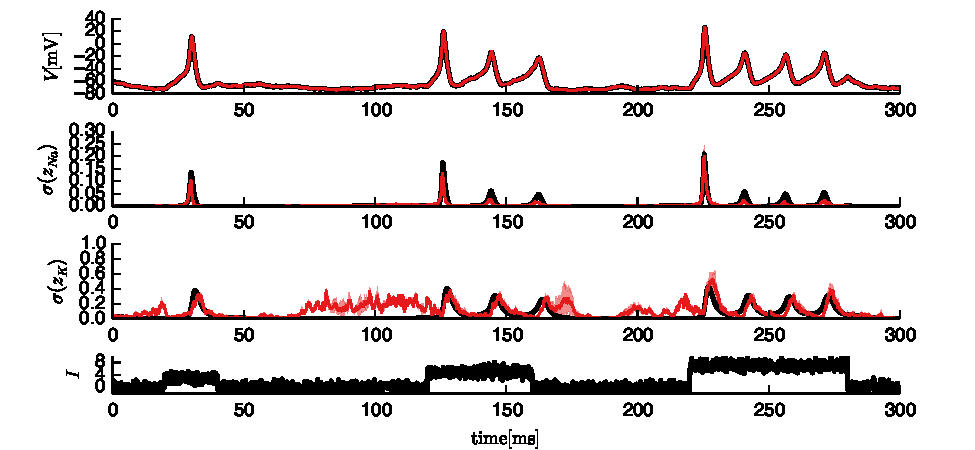
\includegraphics[width=\textwidth]{figure1}
  \end{subfigure}
  \\
  \begin{subfigure}[T]{2in}
      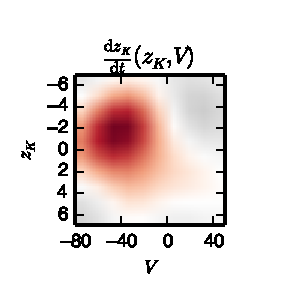
\includegraphics[width=\textwidth]{dk_dt}
  \end{subfigure}

\vspace{-.5em}
\caption{}
\label{fig:figure1}
\vspace{-1.25em}
\end{figure}


\section{Learning with particle MCMC} 
The task of learning the channel dynamics models can be naturally decomposed into three steps: 
\begin{enumerate}
\item[(i)] Infer the membrane potential and channel states given estimates of the channel conductances and the dynamics functions,
\item[(ii)] Infer the channel densities given the membrane potential and the open fractions, 
\item[(iii)] Learn the dynamics functions given the estimates of the channel states.
\end{enumerate}

The first step can be implemented with a particle Gibbs with ancestor resampling (PGAS) kernel \cite{Lindsten-2014}, the second step is a constrained Bayesian linear regression, and the third is a standard Gaussian process regression problem. 

\bibliographystyle{imsart-nameyear}
{\small \bibliography{draft}}

\clearpage

\appendix
\section{A simpler approach that could be useful for initialization}
The nonlinear dynamical system model poses significant inferential problems. As an alternative, we could relax the assumption that the latent states follow a dynamical system and instead assume they are drawn from a Gaussian process that enforces our temporal smoothness constraint. The resulting model would be,
\begin{align*}
\ln g_c &\sim \distNormal(\mu_g, \sigma_g^2) \text{ or } g_c \sim \distGamma(\alpha_g, \beta_g), \\
\bz_c(t) &\sim \mathcal{GP}(\boldsymbol{0}, K(t,t')), \\
\bV &\sim p(V_0) \prod_{t=1}^T p(V_t \given \mu_V(t), \sigma_V^2), \\
\mu_V(t) &= V_{t-1} + \Delta t \sum_{c} g_c \cdot \sigma(z_c(t)) \cdot (V_{t-1}-E_c).
\end{align*}

This model is amenable to simple Gibbs sampling where we sample the~$\bz_c(t)$'s using elliptical slice sampling. Under a Gaussian observation model, the conditional distribution of~$\bV$ is a Gaussian linear dynamical system that may be sampled with a forward-backward algorithm. It's not quite the same as the standard iteration since the coefficients of the dynamical system are changing over time. \TODO{Can we just write~$p(\bV)$ as a multivariate Gaussian?}

\begin{align}
p(V \given z) &= \prod_t p(V_t \given V_{t-1} +  dV/dt(z_t, V_{t-1}) \\
p(z) &= \distNormal(0, K(t,t')). \\
\log p(z) &\propto -\frac{1}{2} z^\trans K^{-1} z  \\
K_{t,t'} &= \exp\{-\frac{1}{2} (t-t')^2/\tau^2 \} + \sigma^2 
\end{align}


\end{document}

   
